\subsection{Piping package}

In questa sezione descriveremo il package \textbf{piping}.

Questo package contiene le implementazioni che permettono di
assemblare una \emph{pipeline}, attraverso la composizione di un
numero quanto si voglia di filtri. Descriveremo i filtri che abbiamo
implementato e come \`e possibile crearne di nuovi.

\subsubsection*{Supplied Abstractions}

Le astrazioni fornite da questo package sono le seguenti:
\begin{itemize}
\item fornire un \emph{template} di filtro, componente atomica per la
  composizione di una \emph{pipeline}. Questo template implementa
  tutto il comportamento necessario affinch\`e possa essere combinato,
  lasciando all'implementatore il compito di codificare la logica che
  caratterizza il filtro che stiamo modellando.
\item fornire un insieme di filtri gi\`a implementati necessari alla
  realizzazione dei requisiti nella sezione
  \ref{section:use-cases}. Questi filtri permettono di generare la
  rappresentazione grafica e testuale di un grafo, di applicare una
  ricerca \emph{DFS}, di applicare l'algoritmo di Tarjan e trasformare
  un grafo collassando le sue sorgenti in una unica.
\item facilitare la creazione dei precedenti filtri attraverso una
  \emph{factory}, in modo da disaccoppiare il codice client dei filtri
  dalle classi specifiche. A differenza di quanto implementato per i
  realizzatori del contratto \emph{Vertex} (vedi
  \ref{subsection:model-supplied-abstractions}), non si vuole
  nascondere le classi che implementano le varie caratterizzazioni di
  filtro, quindi \`e possibile sia utilizzare la factory sia creare i
  filtri utilizzando i rispettivi costruttori.
\item catturare ed esporre il concetto di \emph{listener}, mediante il
  quale \`e possibile essere notificati tramite degli eventi durante
  la computazione. Questi eventi sono modellati tramite messaggi
  definiti in un contratto dedicato e possono essere inviati sia dal
  template che modella il filtro, sia dalla logica che caratterizza il
  comportamento che differienzia un filtro da un altro. Attraverso un
  listener \`e possibile assemblare la propria pipeline ed eseguire
  non solo le trasformazioni che questa produce, ma anche della logica
  quando determinati eventi accadono. Questo \`e uno strumento molto
  potente in quanto permette di essere ortogonali alla pipeline e aver
  un maggior grado di controllo sull'intera computazione.
\end{itemize}

\subsubsection*{Class diagram}
Il diagramma rappresentato in figura \ref{fig:piping-package-classes}
rappresenta i concetti implementati in questo package. Procediamo con
ordine nel descrivere le idee principali catturate da ogni classe:

\begin{figure}
  \centering
  % 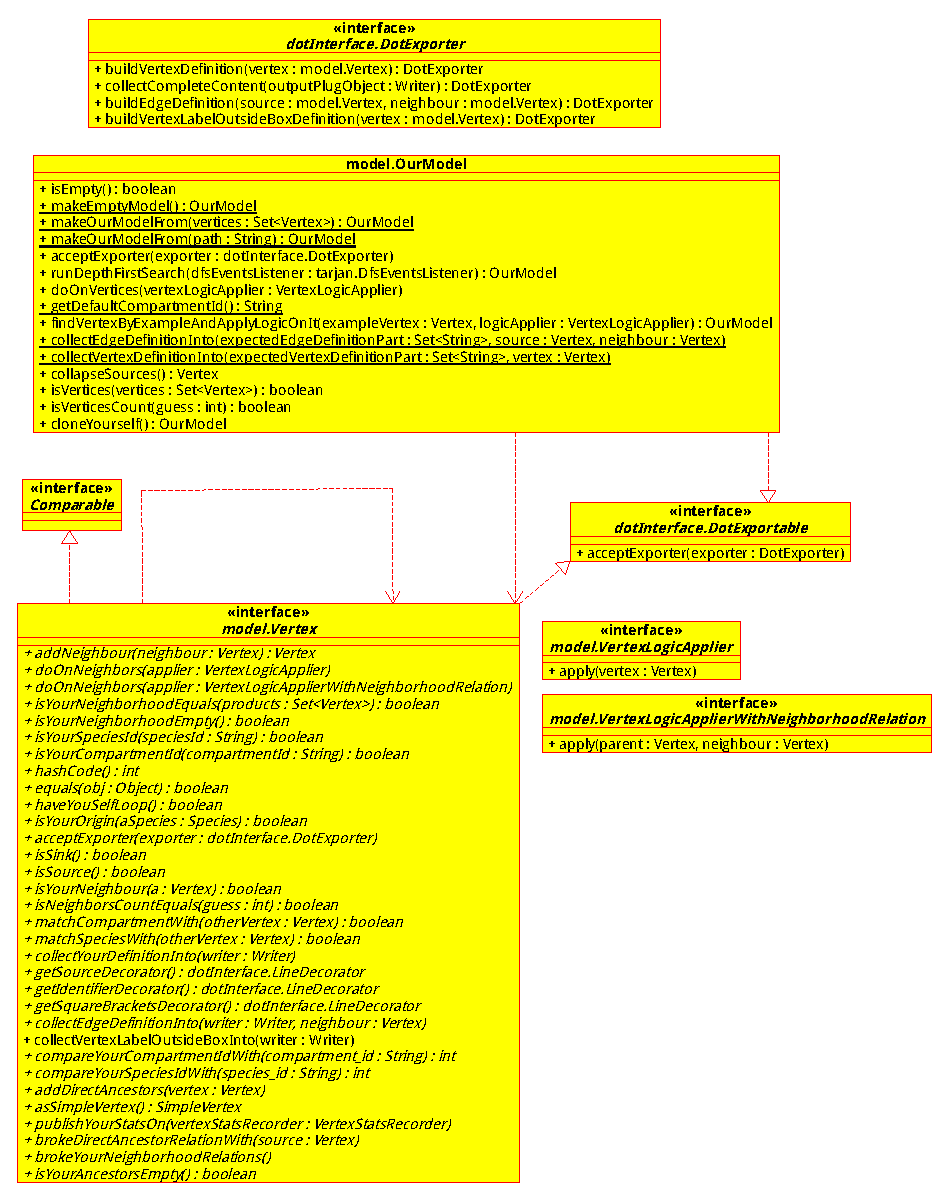
\includegraphics{packages/vertex-interface-class-diagram.eps} 
  \caption{Piping package's classes}
  \label{fig:piping-package-classes}
\end{figure}

\begin{paragraph}{PipeFilter}
  Abbiamo cercato di formalizzare in modo preciso la pi\`u piccola
  unit\`a atomica capace di eseguire una computazione all'interno di
  una sequenza pi\`u grande. Questo ci ha portato alla definizione
  della classe astratta \emph{PipeFilter}. Aver introdotto questa
  classe ci ha permesso di rendere il codice molto flessibile e
  trasparente, nonch\`e molto pi\`u facile da implementare.

  Questa classe, come abbiamo detto nei paragrafi precedenti, in
  realt\`a rappresenta solo un \emph{template} del concetto di filtro
  e non di un filtro che esegue una trasformazione sull'istanza di
  input. Le sue responsabilit\`a sono di poter assemblare una sequenza
  di filtri, utilizzando l'idea alla base della costruzione di una
  lista concatenata, ed eseguire la computazione, eventualmente
  propagando la richiesta di esecuzione a tutti i filtri che si sono
  assemblati.

  Quanto detto nel precedente paragrafo \`e stato molto semplice da
  implementare avendo data a \emph{PipeFilter} una struttura
  ricorsiva: per costruire una pipeline con due filtri \`e sufficiente
  costruirli, dare la relazione di precedenza che identifica la
  pipeline, e sul filtro pi\`u esterno invocare la richiesta di
  esecuzione. Il primo filtro che riceve tale richiesta, controlla se
  il filtro che lo precede \`e istanziato: se lo \`e allora si delega
  la richiesta di esecuzione, altrimenti, o successivamente la
  terminazione dell'esecuzione di tutti gli eventuali filtri
  precedenti, si esegue la trasformazione che caratterizza il filtro
  corrente che ha ricevuto per primo la richiesta. Inoltre, data la
  natura ricorsiva di \emph{PipeFilter}, \`e possibile comporre una
  pipeline i cui filtri sono a loro volta pipeline, oppure un mix di
  pipeline e filtri.

  L'esecuzione di una pipeline riceve come istanza di input un grafo
  codificato da un oggetto di tipo \emph{OurModel}, ed eventualmente
  un listener, questa istanza viene propagata al filtro che non ha
  predecessori. Quest ultimo esegue la sua trasformazione e ritorna un
  nuovo grafo, che diventer\`a instanza di input del suo
  successore. Si applica questa di regola di esecuzione fino a che il
  filtro pi\`u esterno della pipeline, ovvero quello che per primo ha
  ricevuto la richiesta di esecuzione, ricever\`a a sua volta una
  instanza di input, eseguir\`a la computazione e restituir\`a il
  grafo finale.

\end{paragraph}

\begin{paragraph}{Concrete \emph{PipeFilter}s}
  Come abbiamo detto, \emph{PipeFilter} rappresenta solo un
  \emph{template}: il comportamento che vogliamo dare ad ogni filtro
  deve essere codificato in una classe concreta che "completa" tale
  template. In realt\`a non \`e molto il lavoro che si lascia da
  scrivere. Per completare il template \`e sufficiente
  l'implementazione di un metodo astratto, che ha come parametri il
  grafo di input e deve ritornare una grafo utilizzato come input per
  il filtro successivo.

  Tutti i filtri che abbiamo implementato in questa libreria
  compongono il comportamento esposto da altri oggetti, fornendo nella
  maggior parte dei casi le implementazioni di \emph{hook
    methods}\footnote{aggiungere qui riferimento bibliografico al
    volume del Pree}, per ottenere la caratterizzazione desiderata.

  Il primo filtro concreto che abbiamo introdotto \`e stato
  \emph{PrinterPipeFilter}, il quale produce una rappresentazione
  grafica, producendo un documento compilabile con il programma
  \emph{dot}\footnote{aggiungere qui riferimento bibliografico alla
    libreria graphviz}. Questo filtro non apporta nessuna
  trasformazione al grafo di input e lo restituisce cosi come lo ha
  ricevuto. Per adempiere alla sua responsabilit\`a, questo filtro
  costruisce un esportatore (come descritto in \footnote{aggiungere
    qui il riferimento alla sezione del package dotInterface, ancora
    non l'ho descritto}) per visitare il grafo e collezionare tutte le
  informazioni necessarie per costruire il documento \emph{dot}.

  Il secondo filtro concreto che abbiamo introdotto \`e stato
  \emph{DfsPipeFilter}, il quale esegue una visita \emph{DFS} sul
  grafo di input e ritorna un grafo contenente solo il sottoinsieme di
  archi visitati. Concatenando come successore un filtro di tipo
  \emph{PrinterPipeFilter} sar\`a possibile visualizzare l'albero
  \emph{DFS} che rappresenta la visita eseguita.

  Il terzo filtro concreto che abbiamo introdotto \`e stato
  \emph{TarjanPipeFilter}, il quale applica l'algoritmo di Tarjan per
  la ricerca delle componenti fortemente connesse sul grafo di
  ingresso e restituisce un nuovo \emph{dag} composto dalle componenti
  identificate. \`E importante sottolineare la potenza di aver
  strutturato il codice nel modo pi\`u generico possibile, ovvero il
  grafo prodotto da questo filtro non ha come vertici dei semplici
  \emph{SimpleVertex}, bensi degli oggetti che caratterizzano le
  componenti fortemente connesse. In questo modo possiamo continuare
  ad inviare gli stessi messaggi, ad esempio componendo ancora un
  filtro \emph{PrinterPipeFilter}, ma ottenere una rappresentazione
  diversa rispetto a quella che si otterebbe dato un grafo "semplice".

  Il quarto filtro concreto che abbiamo introdotto \`e stato
  \emph{SourcesCollapserPipeFilter}, il quale permette di collassare
  tutte le sorgenti ed introdurne una nuova ed unica. Il nuovo grafo
  viene restituito per eventuali computazioni successive.

  Gli ultimi filtri concreti che abbiamo introdotto sono stati
  \emph{PlainTextStatsPipeFilter} e
  \emph{ConnectedComponentInfoPipeFilter}. Questi hanno la
  responsabilit\`a di produrre una rappresentazione testuale del grafo
  in input, producendo il primo un output tabellare, il secondo una
  serializzazione di una struttura dati che mantiene delle
  informazioni sulle componenti fortemente connesse, consultabili
  utilizzando il relativo programmetto \emph{ResultViewer}.

\end{paragraph}

\begin{paragraph}{PipeFilterComputationListener}
  Il concetto di listener \`e molto simile a quello di \emph{Observer}
  come descritto in \footnote{aggiungere qui riferimento bibliografico
    a Design Patterns}, anche se nella nostra implementazione non
  dobbiamo notificare di un cambiamento, bensi notificare che \`e
  accaduto un determinato evento. Questi eventi sono modellati come
  messaggi nell'interfaccia \emph{PipeFilterComputationListener} e per
  adesso siamo interessati alla notifica dell'inizio e della fine
  della computazione di ogni filtro.

  L'utilit\`a dei listener risiede nella possibilit\`a di ricevere
  degli argomenti inviati dal mittente della notifica ed essere
  elaborati per implementare le funzionalit\`a desiderate. Questi
  argomenti aggiuntivi possono essere relativi non solo ad uno
  specifico filtro, bensi ad un insieme di filtri, in quanto per tutta
  la durata della pipeline si usa lo stesso listener.Un esempio \`e
  \emph{PlainTextInfoComputationListener}, il quale colleziona in una
  mappa, per ogni filtro, delle informazioni che verranno utilizzate
  successivamente per produrre una rappresentazione testuale del
  grafo. Queste informazioni vengono raccolte in un oggetto dapprima
  nell'esecuzione di un filtro \emph{PlainTextStatsPipeFilter}, quando
  questo termina il suo compito, invia un messaggio al listener che la
  computazione \`e terminata, allegando come argomento l'oggetto con
  le informazioni. Questo ci ha permesso di applicare trasformazioni e
  trattare i risultati di queste in modo collettivo, senza doverle
  comporre a computazione terminata.


\end{paragraph}

